\documentclass[aspectratio=169, 10pt]{beamer}
\usetheme{Madrid}
\usecolortheme{default}
\usepackage{tikz}
\usetikzlibrary{shapes.geometric, arrows.meta, positioning, calc}
\usepackage{amsmath}

\title[NS-ARC Architecture]{NS-ARC: Neuro-Symbolic Joint Embedding Predictive Architectures}
\subtitle{Bridging Neural Connectivity with Rule-Based Programmatic Latents}
\author[Model-JEPA]{Model-JEPA Experimentation Project}
\date{\today}

\begin{document}

\frame{\titlepage}

\begin{frame}{The Need: Why ARC Breaks Standard Deep Learning}
    \textbf{The Problem Context:}
    François Chollet's Abstraction and Reasoning Corpus (ARC) evaluates True General Intelligence. Standard Deep Learning models (like CNNs or Vision Transformers) fail systematically on ARC due to fundamental architectural flaws:
    \vspace{0.3cm}
    \begin{itemize}
        \item \textbf{Generative Blurriness:} AutoEncoders and Diffusion models operate continuously. When forced to deduce rigid discrete logic (e.g. ``Move square 3 pixels left''), they hallucinate and smear pixels.
        \item \textbf{Semantic Smearing:} Neural networks blend entire images into massive, single continuous vectors, utterly destroying object-level independence and symbolic relationships.
    \end{itemize}
\end{frame}

\begin{frame}{The Novel Input: NS-ARC Paradigm}
    \textbf{Our Core Solution:} 
    A Neuro-Symbolic architecture designed specifically to extract physics and logic purely mathematically, without requiring human-labeled objects.
    
    \vspace{0.3cm}
    \textbf{Novel Interventions:}
    \begin{enumerate}
        \item \textbf{Reconstruction-Free JEPA:} Eliminates blurry pixel generation. We predict logical states inside an abstract energy-bound hidden dimension.
        \item \textbf{Harmonic Slot Attention:} Dynamically detects and segregates distinct objects entirely unsupervised.
        \item \textbf{Vector Quantization (VQ) Bottlenecks:} Forcibly translates fuzzy continuous objects into rigid, codebook-verified programmatic routines.
    \end{enumerate}
\end{frame}

\begin{frame}{Proposed Architecture (Mathematical Pathway)}
    \begin{center}
    \resizebox{0.95\linewidth}{!}{
    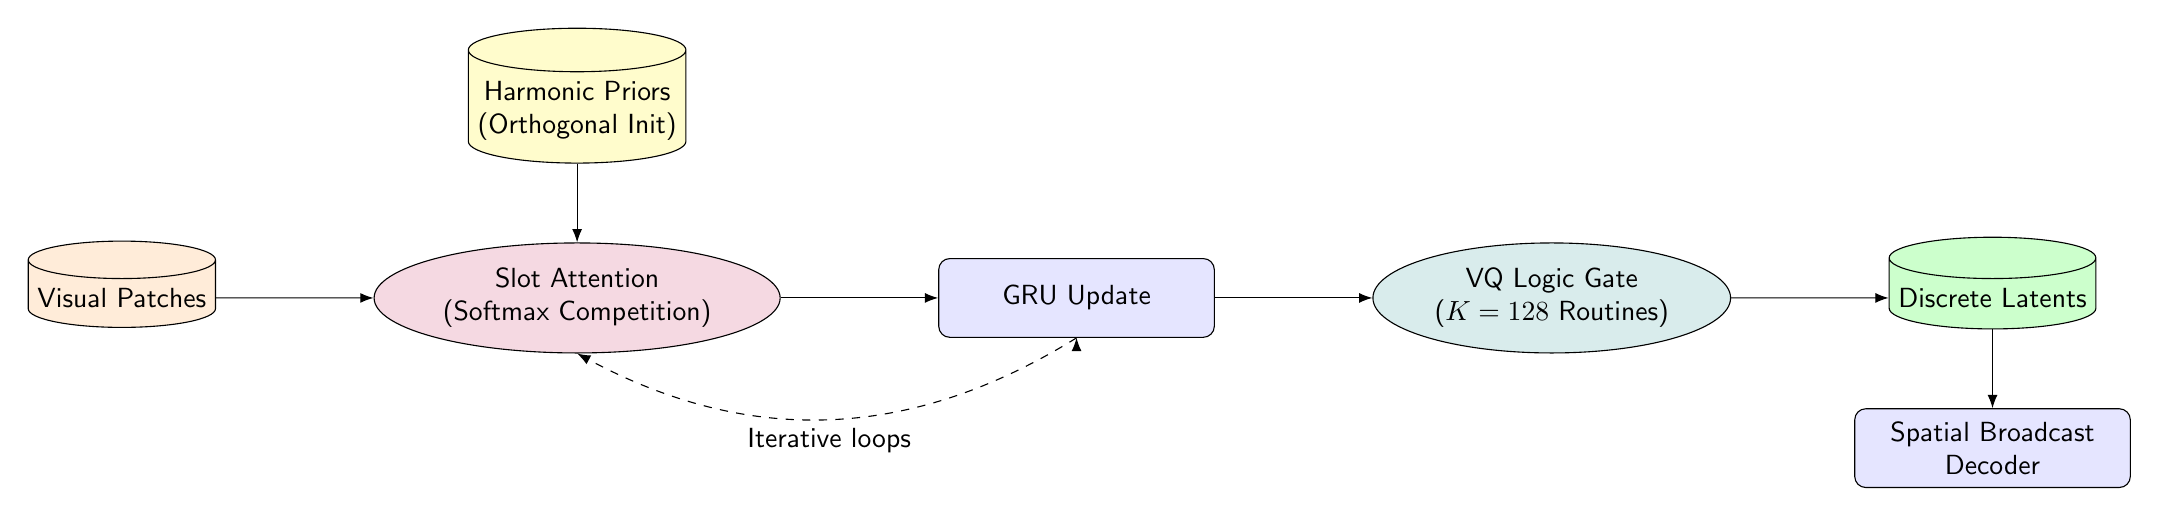
\begin{tikzpicture}[
        >=Latex, node distance=1cm and 2cm, font=\sffamily,
        data/.style={draw, cylinder, shape aspect=0.2, shape border rotate=90, minimum width=2cm, minimum height=1cm, align=center, fill=orange!15},
        block/.style={draw, rectangle, rounded corners, minimum width=3.5cm, minimum height=1cm, align=center, fill=blue!10},
        attn/.style={draw, ellipse, minimum width=3cm, minimum height=1cm, align=center, fill=purple!15}
    ]
    \node[data] (patches) {Visual Patches};
    \node[attn, right=of patches] (compete) {Slot Attention\\(Softmax Competition)};
    \node[data, above=1cm of compete, fill=yellow!20] (priors) {Harmonic Priors\\(Orthogonal Init)};
    \node[block, right=of compete] (gru) {GRU Update};
    \node[attn, right=of gru, fill=teal!15] (vq) {VQ Logic Gate\\($K=128$ Routines)};
    \node[data, right=of vq, fill=green!20] (zdisc) {Discrete Latents};
    \node[block, below=1cm of zdisc] (decoder) {Spatial Broadcast\\Decoder};

    \draw[->] (patches) -- (compete);
    \draw[->] (priors) -- (compete);
    \draw[->] (compete) -- (gru);
    \draw[->] (gru) -- (vq);
    \draw[->] (vq) -- (zdisc);
    \draw[->] (zdisc) -- (decoder);
    \draw[->] (gru.south) edge[bend left=30, dashed] node[below] {Iterative loops} (compete.south);
    \end{tikzpicture}
    }
    \end{center}
\end{frame}

\begin{frame}{Architectural Mechanics: Forcing Discrete Logic}
    How do we mathematically force a neural network to perform discrete algorithms?
    \vspace{0.3cm}
    \begin{block}{1. Object Separation (Attention over Slots)}
        We invert Standard Attention. By running the $\text{Softmax}$ over the $K$ slots instead of the spatial dimensions, slots actively compete. If Slot 1 binds to an object, the math steals gradients from Slot 2, forcing independent object routing.
    \end{block}
    \begin{block}{2. Logic Constraining (The Straight-Through VQ Snap)}
        Instead of decoding directly, continuous object vectors $Z_{cont}$ are dragged to the nearest integer state inside a predefined Codebook Matrix organically evolving via gradient descent. Vague concepts solidify into strict states.
    \end{block}
\end{frame}

\begin{frame}{Current Training Challenges 1: Spatial Monopoly}
    \textbf{The Obstacle: "Winner-Take-All" Collapse}
    Because ARC backgrounds comprise 95\% of a grid's spatial mass, the Slot Attention mechanism realized it could brutally exploit the Cross-Entropy loss by instructing \textit{a single slot} to output a uniform background color everywhere, totally shutting down other slots and permanently ignoring the tiny structural shapes (orange/red logic blocks).
    
    \vspace{0.2cm}
    \textbf{The Resolution: Foreground Weighted Gradients}
    Implemented massive gradient inflation. Any physical pixel $Y \neq 0$ (foreground shape) evaluates at a penalty multiplier of $50.0\times$. 
    \begin{equation}
        \mathcal{L} = \mathbb{E}\left[ -\log(p) \cdot \begin{cases} 50.0 & Y_{true} > 0 \\ 1.0 & Y_{true} = 0 \end{cases} \right] 
    \end{equation}
    This destroys the Winner-take-all exploit, forcing dead slots to resurrect.
\end{frame}

\begin{frame}{Current Training Challenges 2: Informational Collapse}
    \textbf{The Obstacle: Harmonics Erosion}
    We initialize slots via Harmonic Disentanglement (polar-opposite Trigonometric waves). However, a standard AdamW optimizer's initial shockwaves inside the Iterative GRU systematically homogenized these beautiful priors, averaging them into a single blob by Epoch 80.
    
    \vspace{0.2cm}
    \textbf{The Resolution: VICReg \& Warmup Curriculum}
    \begin{itemize}
        \item \textbf{OneCycleLR Warmup:} Prevents initial gradient explosions, allowing the GRU to slowly ease out of its Harmonic start states without breaking them.
        \item \textbf{VICReg Variance Hinge:} Structurally penalizes the network if the Standard Deviation across the $D$-dimensional Slot dimension drops below a margin $\gamma$. Forces informational independence.
    \end{itemize}
\end{frame}

\begin{frame}{Conclusion and Roadmap}
    Our NS-ARC system elegantly merges powerful neural-spatial routing with strict rule-based symbolic extraction. 
    
    \vspace{0.3cm}
    \textbf{Immediate Roadmap:}
    \begin{itemize}
        \item Track Foreground Weighted validation accuracy past Epoch 150.
        \item Monitor the VQ Commitment Loss tracking logic saturation. 
        \item Dynamically scale the VQ Codebook from $K=128 \rightarrow 512$ via network surgery to inject capacity for complex physics algorithms without causing catastrophic forgetting of baseline colors/shapes.
    \end{itemize}
\end{frame}

\end{document}
